\documentclass[10pt, twoside]{article}
\usepackage{main}

% Aquí empieza el documento{{{
\begin{document}

%\maketitle
\thispagestyle{fancy}

% Carátula {{{
\begin{center}
	$1^{\text{ER}}$ LABORATORIO DE FÍSICA $2$
	%Informe del Laboratorio N° 1
\end{center}

\noindent
\begin{tikzpicture}
	\tikzmath
	{
		coordinate \xMa;
		\xMa = (\textwidth-1.6pt,0);
	}
	\draw [ultra thick](0,0) rectangle ++(\xMax*0.8,-5)
		++(0.25,0)
		rectangle (\xMax,0);

	\draw(2,-.5) node {Título del laboratorio};
	\draw({(\xMax*0.8+\xMax)/2},-.5) node {NOTA};
\end{tikzpicture}

\bigskip
\bigskip
\bigskip
\noindent
%\begin{tikzpicture}
	%\tikzmath
	%{
		%coordinate \xMa;
		%\xMa = (\textwidth-0.4pt,0);
	%}
	%\foreach \x in {0, ..., 5}
	%{
		%\draw ({\x*\xMax/6},0) rectangle ++(\xMax/6,0.75);
	%}
	%\draw (0.62,0.4) node {\textbf{Fecha}}
		%++(\xMax/3,0) node {\textbf{Hora}}
		%++(\xMax/3,0)++(0.4,0) node {\textbf{Ambiente}}
		%;
%\end{tikzpicture}

\bigskip
\bigskip
\noindent
\begin{tikzpicture}
	\tikzmath
	{
		coordinate \xMa;
		\xMa = (\textwidth-0.4pt,0);
	}
	\foreach \y in {0,1}
	{
		\draw (0,\y) rectangle +(\xMax*0.5,-1)
			++(\xMax*0.5,0) rectangle ++(\xMax*0.25,-1)
			+(0,1) rectangle (\xMax,\y-1);
	}
	\draw (\xMax*0.25,0.7) node {\textbf{Integrantes}}
		++(\xMax*0.38,0) node {\textbf{Código}}
		++(\xMax*0.25,0) node {\textbf{Participación}}
		++(0,-0.4) node {\textbf{(\%)}}
		;
	\draw (\xMax*0.25,0.7-1) node {Alberto Oporto Ames}
		++(\xMax*0.38,0) node {$201810518$}
		++(\xMax*0.25,0) node {100\%}
		;
\end{tikzpicture}
% }}}

\newpage

\section{EXPERIENCIA A:Observación de superficies equipotenciales y líneas de
campo eléctrico}%

\subsection{OBJETIVOS}%

Escribir en una tabla las coordenadas de los puntos en los que
el voltaje es el mismo.

\subsection{PROCEDIMIENTO Y ANÁLISIS}%
Datos:
\begin{itemize}
	\item Coordenadas
	\item Voltajes
	\item Cargas
	\item Constante dieléctrica del agua
\end{itemize}

\[
	U = 0.6cm
\]

\begin{table}[H]
	\centering
	\caption{Coordenadas}
	\label{tab:coordenadas}
	\begin{tabular}{c|c||c|c||c|c||c|c}
		\multicolumn{2}{c||}{$2V$}
		&\multicolumn{2}{c||}{$3V$}
		&\multicolumn{2}{c||}{$4V$}
		&\multicolumn{2}{c}{$4.5V$}\\
		\hline
		\hline
		x & y & x & y & x & y & x & y\\
		\hline
		$-10U$ & $1U$ & $-6.5U$ & $-5U$ & $4U$ & $7U$ & $10U$ & $9U$\\
		\hline
		$-12U$ & $-1U$ & $-5U$ & $-1U$ & $4U$ & $5U$ & $13U$ & $12U$\\
		\hline
		$-14U$ & $-2U$ & $-4U$ & $1U$ & $3U$ & $3U$ & $5U$ & $-10U$\\
		\hline
		$-16U$ & $-3.5U$ & $-3U$ & $5U$ & $2U$ & $0U$ & $4U$ & $-5U$\\
		\hline
		$-18U$ & $-4U$ & $-2U$ & $8U$ & $-2U$ & $-2U$ & $4U$ & $-2U$\\
		\hline
		$-8U$ & $4U$ & $-2U$ & $12U$ & $2U$ & $-4U$ & $4U$ & $0U$\\
		\hline
		$-7U$ & $7U$ & $-6U$ & $-10U$ & $1.5U$ & $-5U$ & $5U$ & $3U$\\
		\hline
		$-7.5U$ & $10U$ & $-7U$ & $-7U$ & $2U$ & $-9U$ & $7U$ & $6U$\\
		\hline
	\end{tabular}
\end{table}

\begin{figure}[H]
	\centering
	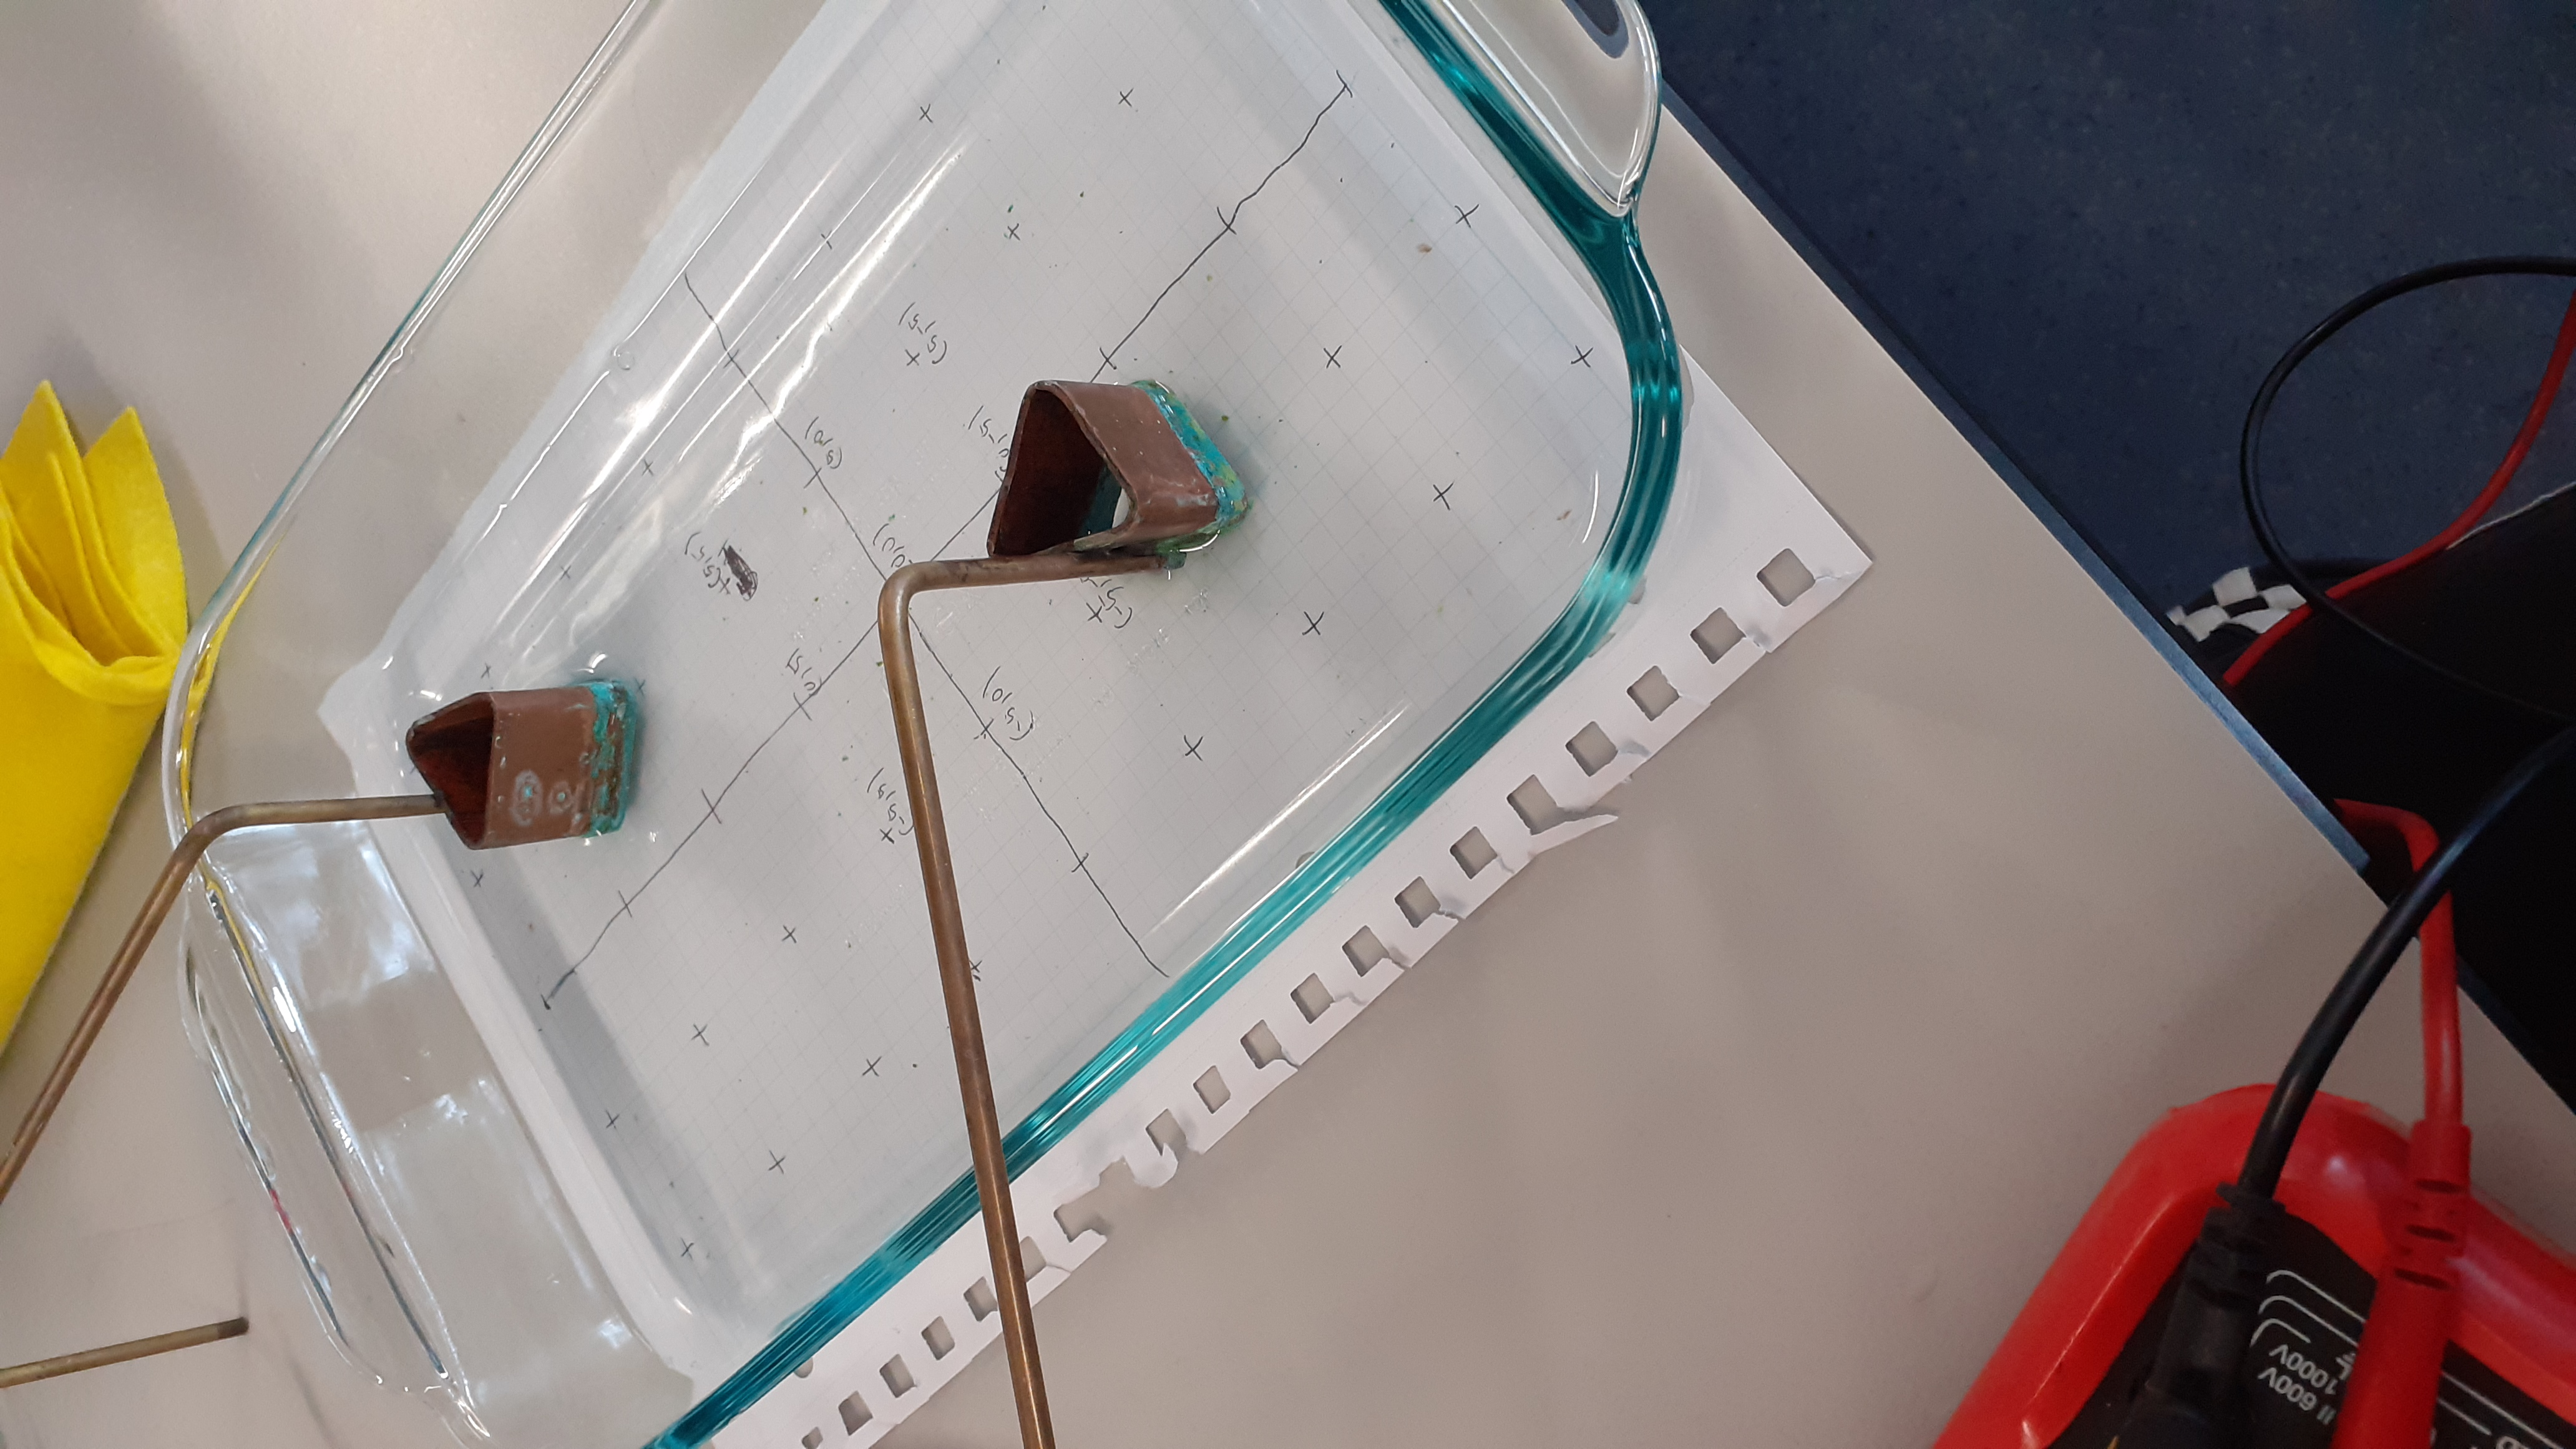
\includegraphics[width=0.8\linewidth, angle=-90]{20190917_152938.jpg}
	\caption{Electrodos en una bandeja}%
	\label{fig:bandeja}
\end{figure}

Llené una bandeja con agua y sal,
puse los electrodos (positivo a la derecha y negativo a la izquierda)
medí los puntos con el mismo voltaje
y escribí sus coordenadas en una tabla.

\subsection{COMENTARIOS Y OBSERVACIONES}%

Tuve que tomar datos dos veces,
dibujar mis ejes de coordenadas 3 veces
y por unos días pensé que había perdido mi hoja con los datos.

\subsection{CUESTIONARIO}%

\begin{enumerate}[label=\roman*]
	\item Dibuja las líneas de campo y las líneas equipotenciales en la hoja
		cuadriculada, no olvidar de dibujar el contorno y la posición de los
		electrodos usados.
	\begin{figure}[H]
		\centering
		\includegraphics[width=\linewidth]{lineas}
		\caption{Líneas}%
		\label{fig:lineas}
	\end{figure}
	\item Aproximar la carga de los electrodos al centro de los mismos,
		mostrar el cálculo para obtener la carga total del electrodo.
		\begin{align*}
			\intertext{Constante dieléctrica del agua}
			k &= 80
			\intertext{Posiciones de los electrodos}
			P_- &= <-12;6.5>U\\
			P_+ &= <10;0>U
			\intertext{Dos puntos con el mismo voltaje $(V=4.5V)$}
			P_1 &= <13,12>U\\
			P_2 &= <5,-10>U\\
			\\
			V_1 &= \frac{k_0}{k} \frac{Q_-}{r_{1-}} + \frac{k_0}{k} \frac{Q_+}{r_{1+}} = 4.5V\\
			V_2 &= \frac{k_0}{k} \frac{Q_-}{r_{2-}} + \frac{k_0}{k} \frac{Q_+}{r_{2+}} = 4.5V\\
			\\
			V_1 &= \frac{Q_-}{r_{1-}} + \frac{Q_+}{r_{1+}} = 4.5V \frac{k}{k_0} \\
			V_2 &= \frac{Q_-}{r_{2-}} + \frac{Q_+}{r_{2+}} = 4.5V\frac{k}{k_0}\\
			\\
			\frac{Q_-}{r_{1-}} \frac{r_{1+}}{r_{2+}}+
			\frac{Q_+}{\cancel{r_{1+}} } \frac{\cancel{r_{1+}} }{r_{2+}}
			&= 4.5V \frac{k}{k_0} \frac{r_{1+}}{r_{2+}}\\
			\frac{Q_-}{r_{2-}} + \frac{Q_+}{r_{2+}} &= 4.5V\frac{k}{k_0}\\
			\\
			\frac{Q_-}{r_{1-}} \frac{r_{1+}}{r_{2+}}+
			\frac{Q_+}{r_{2+}}
			&= 4.5V \frac{k}{k_0} \frac{r_{1+}}{r_{2+}}\\
			\frac{Q_-}{r_{2-}} + \frac{Q_+}{r_{2+}} &= 4.5V\frac{k}{k_0}\\
			\\
			\frac{Q_+}{r_{2+}}
			&= 4.5V \frac{k}{k_0} \frac{r_{1+}}{r_{2+}}
			-\frac{Q_-}{r_{1-}} \frac{r_{1+}}{r_{2+}}\\
			\frac{Q_+}{r_{2+}} &= 4.5V\frac{k}{k_0}-\frac{Q_-}{r_{2-}} \\
			\\
			4.5V \frac{k}{k_0} \frac{r_{1+}}{r_{2+}}
			-\frac{Q_-}{r_{1-}} \frac{r_{1+}}{r_{2+}}
			&= 4.5V\frac{k}{k_0}-\frac{Q_-}{r_{2-}} \\
			%
			4.5V \frac{k}{k_0} \frac{r_{1+}}{r_{2+}}
			-4.5V\frac{k}{k_0}
			&= \frac{Q_-}{r_{1-}} \frac{r_{1+}}{r_{2+}}
			-\frac{Q_-}{r_{2-}}\\
			4.5V \frac{k}{k_0} \left(\frac{r_{1+}}{r_{2+}}
			-1 \right)
			&= \frac{Q_-}{r_{1-}} \left(\frac{r_{1+}}{r_{2+}}
			- \frac{1}{r_{2-}} \right)\\
			\frac
			{
				4.5V \frac{k}{k_0} \left(\frac{r_{1+}}{r_{2+}}
				-1 \right)
			}
			{
				\left(\frac{r_{1+}}{r_{2+}} - \frac{1}{r_{2-}}  \right)
			}
			&= \frac{Q_-}{r_{1-}}\\
			Q_- &=
			\frac
			{
				4.5V k r_{1-} * \left(\frac{r_{1+}}{r_{2+}}
				-1 \right)
			}
			{
				k_0 \left(\frac{r_{1+}}{r_{2+}} - \frac{1}{r_{2-}} \right)
			}
			\intertext{Distancias}
			r_{1-} &= |P_--P_1| \\
			r_{1-} &= |<-12;6.5>-<13;12>|U\\
			r_{1-} &= |<-25;-5.5>|U\\
			r_{1-} &= \sqrt{25^2+5.5^2}U\\
			r_{1-} &= 25.60U \\
			r_{1-} &= 15.36m*10^{-2}\\
			\\
			r_{1+} &= |P_+-P_1| \\
			r_{1+} &= |<10;0>-<13;12>|U\\
			r_{1+} &= |<-3;-12>|U\\
			r_{1+} &= \sqrt{3^2+12^2}U\\
			r_{1+} &= 12.40U\\
			r_{1+} &= 7.44m*10^{-2}\\
			\\
			r_{2-} &= |P_--P_2| \\
			r_{2-} &= |<-12;6.5>-<5;-10>|U\\
			r_{2-} &= |<-17;16.5>|U\\
			r_{2-} &= \sqrt{17^2+16.5^2}U\\
			r_{2-} &= 23.69U\\
			r_{2-} &= 14.21m*10^{-2}\\
			\\
			r_{2+} &= |P_+-P_2| \\
			r_{2+} &= |<10;0>-<5;-10>|U\\
			r_{2+} &= |<5;10>|U\\
			r_{2+} &= 11.18U\\
			r_{2+} &= 6.70m*10^{-2}
			\intertext{Reemplazando}
			Q_- &=
			\frac
			{
				4.5V k*15.36m*10^{-2} * \left(\frac{7.44m*\cancel{10^{-2}} }{6.70m*\cancel{10^{-2}} }
				-1 \right)
			}
			{
				k_0 \left(\frac{7.44m*\cancel{10^{-2}} }{6.70m*\cancel{10^{-2}} } -
				\frac{1}{14.21m*10^{-2}} \right)
			}\\
			Q_- &=
			\frac
			{
				4.5V 80 *15.36m*10^{-2} * \left(\frac{7.44}{6.70}
				-1 \right)
			}
			{
				9*10^9* \frac{Nm^2}{C^2} \left(\frac{7.44}{6.70} -
				\frac{100}{14.21m} \right)
			}\\
			Q_- &=
			\frac
			{
				4.5 * 80* 9*10^{-11}* 15.36 * 0.11
			}
			{
				-47.41
			}C\\
			Q_- &= -1.15C*10^{-9}
			\\
			\frac{Q_+}{r_{2+}} &= 4.5V\frac{k}{k_0}-\frac{Q_-}{r_{2-}} \\
			\frac{Q_+}{6.70m*10^{-2}} &=
			4.5V\frac{80}{9*10^9 \frac{Nm^2}{C^2} }-\frac{-1.15C*10^{-9}}{14.21m*10^{-2}} \\
			Q_+ &=
			6.70*10^{-2}
			(40*10^{-9}+ 8.09*10^{-9})C \\
			Q_+ &= 3.22C*10^{-9}
		\end{align*}
	\item Escoger $3$ puntos que pertenecen a las líneas equipotenciales
		dibujadas y aproximar el valor de la intensidad de campo
		eléctrico (mostrar los cálculos) y también mostrar la dirección
		aproximada del vector intensidad de campo eléctrico.
		\begin{align*}
			\intertext{Constante dieléctrica del agua}
			k &= 80
			\intertext{Posiciones de los electrodos}
			P_- &= <-12;6.5>U\\
			P_+ &= <10;0>U
			\intertext{Cargas de los electrodos}
			Q_- &= -1.15C*10^{-9}\\
			Q_+ &= 3.22C*10^{-9}
			\intertext{Tres puntos $V=4.5V$}
			P_1 &= <4;-5>U\\
			P_2 &= <4;-2>U\\
			P_3 &= <5;3>U
			\intertext{Campos eléctricos}
			\vec{E}_1 &= \vec{E}_{1-}+\vec{E}_{1+}\\
			\vec{E}_1 &=
			\frac{k_0}{k}
			\frac{Q_-}{r_{1-}^3}*(P_1-P_-)
			+
			\frac{k_0}{k}
			\frac{Q_+}{r_{1+}^3}*(P_1-P_+)\\
			\vec{E}_1 &=
			\frac{k_0}{k}
			\left(
			\frac{Q_-}{r_{1-}^3}*<16;-11,5>
			+
			\frac{Q_+}{r_{1+}^3}*<-6;-5>
			\right)\\
			\vec{E}_1 &=
			\frac{9*\cancel{10^9}}{80}
			\left(
				\frac{-1.15*\cancel{10^{-9}} }{7650.10}*<16;-11,5>
				+
				\frac{3.22*\cancel{10^{-9}} }{476.43}*<-6;-5>
			\right)
			\frac{N}{C}\\
			\vec{E}_1 &=
			\frac{9}{80}
			\left(
				<-0.24;0.17>
				+
				<-4.06;-3.38>
			\right)
			*10^{-2}
			\frac{N}{C}\\
			\vec{E}_1 &=
				<-4.84;-3.61>
			*10^{-3}
			\frac{N}{C}\\
			\\
			\vec{E}_2 &= \vec{E}_{2-}+\vec{E}_{2+}\\
			\vec{E}_2 &=
			\frac{k_0}{k}
			\frac{Q_-}{r_{2-}^3}*(P_2-P_-)
			+
			\frac{k_0}{k}
			\frac{Q_+}{r_{2+}^3}*(P_2-P_+)\\
			\vec{E}_2 &=
			\frac{9*\cancel{10^9}}{80}
			\left(
				\frac{-1.15*\cancel{10^{-9}} }{5947.13}*<16;-8.5>
				+
				\frac{3.22*\cancel{10^{-9}} }{252.98}*<-6;-2>
			\right)
			\frac{N}{C}\\
			\vec{E}_2 &=
			\frac{9}{80}
			\left(
				<-0.31;0.16>
				+
				<-7.64;-2.54>
			\right)
			*10^{-2}
			\frac{N}{C}\\
			\vec{E}_2 &=
			<-8.94;-2.68>
			*10^{-3}
			\frac{N}{C}\\
			\\
			\vec{E}_3 &= \vec{E}_{3-}+\vec{E}_{3+}\\
			\vec{E}_3 &=
			\frac{k_0}{k}
			\frac{Q_-}{r_{3-}^3}*(P_3-P_-)
			+
			\frac{k_0}{k}
			\frac{Q_+}{r_{3+}^3}*(P_3-P_+)\\
			\vec{E}_3 &=
			\frac{9*\cancel{10^9}}{80}
			\left(
				\frac{-1.15*\cancel{10^{-9}} }{5228.66}*<17;-3.5>
				+
				\frac{3.22*\cancel{10^{-9}} }{198.25}*<-5;3>
			\right)
			\frac{N}{C}\\
			\vec{E}_3 &=
			\frac{9}{80}
			\left(
				<-0.37;0.08>
				+
				<-8.12;4.87>
			\right)
			*10^{-2}
			\frac{N}{C}\\
			\vec{E}_3 &=
			<-9.55;5.57>
			*10^{-3}
			\frac{N}{C}
			\intertext{Promedio}
			\vec{E} &= \frac{\vec{E}_1+\vec{E}_2+\vec{E}_3}{3}\\
			\vec{E} &= \frac{<(-4.84-8.94-9.55)+(-3.61-2.68+5.57)>}{3}*10^{-3} \frac{N}{C}\\
			\vec{E} &= \frac{<-23.33;-0.72>}{3}*10^{-3} \frac{N}{C}\\
			\vec{E} &= <-7.78;-0.24> *10^{-3} \frac{N}{C}
			\intertext{Intensidad}
			|\vec{E}| &= \sqrt{7.78^2+0.24^2} *10^{-3} \frac{N}{C} \\
			|\vec{E}| &= 7.7837 *10^{-3} \frac{N}{C}
			\intertext{Dirección}
			\hat{E} &= \frac{\vec{E}}{|\vec{E}|}\\
			\hat{E} &= \frac
			{
				<-7.78;-0.24>
			}
			{
				7.7837
			}\\
			\hat{E} &= -0.9995\hat{\imath} - 0.0307\hat{\jmath}
		\end{align*}
\end{enumerate}

\subsection{CONCLUSIONES}%
Los los electrodos tienen magnitudes de carga diferentes.

\newpage
\section{EXPERIENCIA B:Carga y descarga de un condensador}%

\subsection{OBJETIVOS}%

Grabar con un celular un multímetro y gastar casi toda mi
memoria libre,
intentar saber la resistencia de las resistencias,
y volver a usar un breadboard después de 4 años.

\subsection{PROCEDIMIENTO Y ANÁLISIS}%


\begin{wrapfigure}{R}{0.5\linewidth}
	\centering
	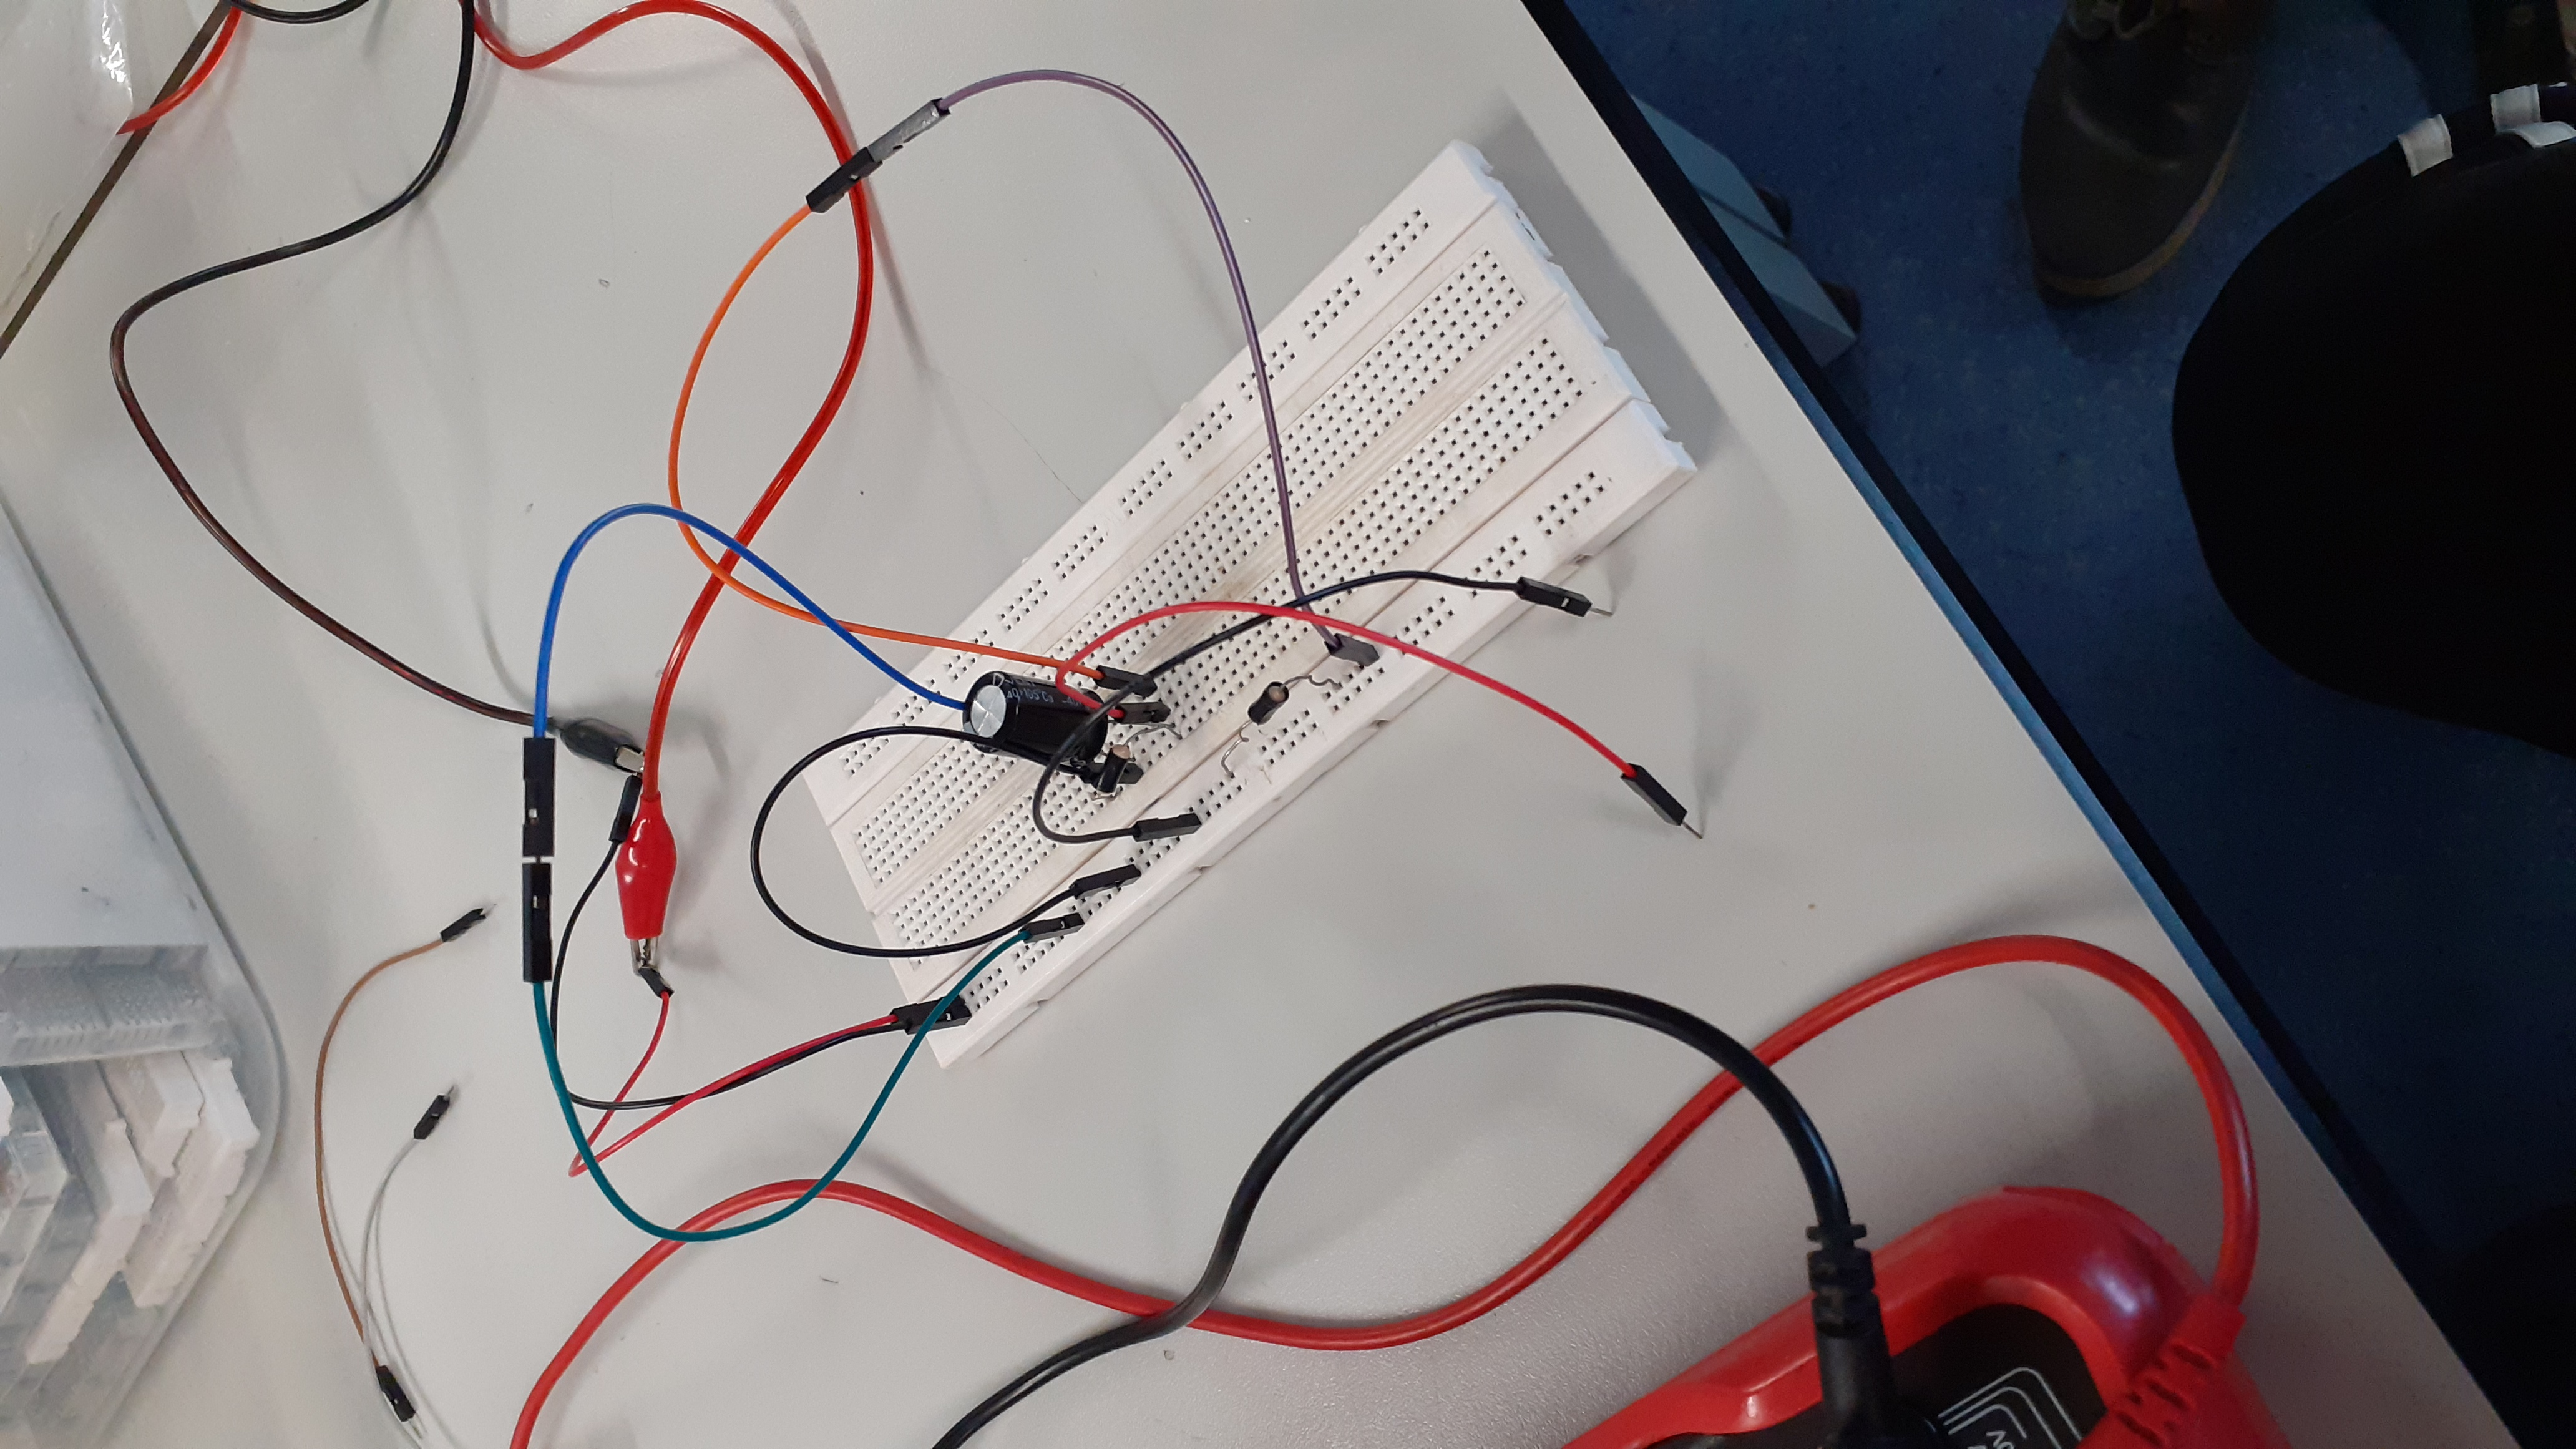
\includegraphics[width=0.9\linewidth, angle=-90]{20190917_163108.jpg}
	\caption{Un Breadboard}%
	\label{fig:bread}
\end{wrapfigure}

Datos:

\begin{itemize}
	\item Voltaje
	\item Tiempo
\end{itemize}

Grabé dos videos con mi celular.

Uno cargando el capacitor y el otro descargándolo.

Después saqué una imagen por cada segundo de ambos videos,
y para cada video escribí en un .csv el tiempo y el voltaje.

Y con ambos .csv hice los gráficos.

\textcolor{white}
{
	aaaaa
	aaaaa
	aaaaa
	aaaaa
	aaaaa
	aaaaa
	aaaaa
	aaaaa
	aaaaa
	aaaaa
	aaaaa
	aaaaa
	aaaaa
	aaaaa
	aaaaa
	aaaaa
	aaaaa
	aaaaa
	aaaaa
	aaaaa
	aaaaa
	aaaaa
	aaaaa
	aaaaa
	aaaaa
	aaaaa
	aaaaa
	aaaaa
	aaaaa
	aaaaa
	aaaaa
	aaaaa
	aaaaa
	aaaaa
	aaaaa
	aaaaa
	aaaaa
	aaaaa
	aaaaa
	aaaaa
}

\pgfplotsset
{
	% Para más argumento habría que poner "n args" a la derecha del /.style
	% Estilo del cuadro
	grafico/.style=
	{
		width=\linewidth,
		height=6cm,
		ymax=10,
		%
		title=\textbf{#1},
		%
		axis y line=left,
		axis x line=bottom,
		axis line style = ultra thick,
		%
		xlabel={Tiempo $(s)$},
		ylabel={Voltaje $(v)$},
		ymajorgrids=true
	},
	% Estilo de la línea del voltaje
	linea/.style=
	{
		color=red,
		ultra thick
	},
	% "Estilo" de la tabla
	table/volt/.style=
	{
		col sep=comma,
		%
		x index=0,
		y index=1
	}
}

\begin{figure}[H]
	\centering

	\begin{tikzpicture}[scale=1, transform shape]
		\begin{axis}[grafico=Carga]
			\addplot[linea] table[volt] {carga.csv};
		\end{axis}
	\end{tikzpicture}
\end{figure}

\begin{figure}[H]
	\centering

	\begin{tikzpicture}[scale=1, transform shape]
		\begin{axis}[grafico=Descarga]
			\addplot[linea] table [volt] {descarga.csv};
		\end{axis}
	\end{tikzpicture}
\end{figure}

\subsection{COMENTARIOS Y OBSERVACIONES}%

No había el medidor logger pro de la guía,
así que tuve que medir el voltaje con un multímetro y mi celular.

\subsection{CUESTIONARIO}%
\begin{enumerate}[label=\roman*]
	\item Mostrar y resolver la ecuación diferencial obtenida al aplicar la
		leyes de Kirchhoff en un circuito $RC$.
		Mostrar la ecuación de voltaje respecto a tiempo que se debería
		obtener de manera teórica.
	\item Comparar las funciones de carga y descarga observadas con las
		funciones obtenidas en el ítem anterior.
		Usar \textbf{PGFPLOTS} para realizar la comparación de las funciones.
	\item Aproximar los valores de la resistencia $R_1$ y $R_2$ utilizando
		las gráficas obtenidas de carga y descarga.
		Utilizar todos los puntos y obtener valores promedio de resistencias.
\end{enumerate}

\subsection{CONCLUSIONES}%

\section{EXPERIENCIA C:Cuantificación del campo magnético}%

\subsection{OBJETIVOS}%

Poner un palo dentro de unos aros y copiar, del logger pro, la magnitud promedio
del campo magnético.

\subsection{PROCEDIMIENTO Y ANÁLISIS}%
Datos
\begin{itemize}
	\item Campo magnético.
\end{itemize}

Medí el campo magnético lejos de la computadora.

Después saqué el promedio del campo magnético dentro de una espira.
Y al final dentro de dos.
\begin{itemize}
	\item Diámetro de las bobinas: $11.2cm$
	\item Distancia entre la primera bobina y la punta del palo: $9.3cm$
	\item Distancia entre las bobinas: $15cm$
	\item Campo magnético default: $0.1438mT$
	\item Campo magnético de una bobina:
		\begin{itemize}
			\item $1.3A$: $1.486mT$
			\item $1.6$: $1.798mT$
			\item $2.9$: $3.125mT$
		\end{itemize}
	\item Campo magnético de dos bobinas:
		\begin{itemize}
			\item $1.3A$: $0.989mT$
			\item $1.6$: $1.183mT$
			\item $2.9$: $2.010mT$
		\end{itemize}
\end{itemize}

\subsection{COMENTARIOS Y OBSERVACIONES}%

Al inicio conecté la bobina con unos cocodrilos.
La intensidad seguía siendo $0A$ y no había campo magnético.

Tenía que usar esos conectores que parecen dispensadores de gasolina.

Al parecer hay menos campo magnético cuando las dos bobinas
están activadas.

Ya había terminado, pero no había medido el diámetro de la bobina.
Tuve que volver a hacer una reserva para medirlo.

Y al final creí que ya tenía todo lo necesario.
Olvidé tomar una foto de la última experiencia.

\subsection{CUESTIONARIO}%
\begin{enumerate}[label=\roman*]
	\item Utilizando las mediciones de campo magnético para una bobina,
		estimar el valor de su número de vueltas $N$.
		\begin{align*}
			B &= \frac{\mu_0I}{2R}N
			\intertext{$1.3A$:}
			B_{1.3} &= \frac{4\pi*10^{-7}*1.3A}{1.12m*10^{-1}}N_{1.3} = (1.486-0.1438)T*10^{-3}\\
			N_{1.3} &= \frac{1,12*10^{-1}*1.3422*10^{-3}}{4\pi*10^{-7}*1.3}\\
			N_{1.3} &= 92.01
			\intertext{$1.6A$:}
			B_{1.6} &= \frac{4\pi*10^{-7}*1.6A}{1.12m*10^{-1}}N_{1.6} = (1.798-0.1438)T*10^{-3}\\
			N_{1.6} &= \frac{1,12*10^{-1}*1.6542*10^{-3}}{4\pi*10^{-7}*1.6}\\
			N_{1.6} &= 92.14
			\intertext{$2.9A$:}
			B_{2.9} &= \frac{4\pi*10^{-7}*2.9A}{1.12m*10^{-1}}N_{2.9} = (3.125-0.1438)T*10^{-3}\\
			N_{2.9} &= \frac{1,12*10^{-1}*2.9812*10^{-3}}{4\pi*10^{-7}*2.9}\\
			N_{2.9} &= 91.62
			\intertext{Promedio}
			N &= \frac{N_{1.3}+N_{1.6}+N_{2.9}}{3} \\
			N &= \frac{92.01+92.14+91.62}{3} \\
			N &= 91.92
		\end{align*}
	\item Utilizando el valor de $N$ hallado en el paso anterior,
		determina el valor teórico en el punto en el que se realizó la medición
		utilizando dos bobinas.
		Compara esto con el valor medido,
		y halla el porcentaje de error respecto al valor teórico.
\end{enumerate}

\subsection{CONCLUSIONES}%

\end{document}
%}}}
